% Contributions are much appreciated, in order to contribute to this project, head over to this repository:
% https://github.com/bshramin/uofa-eng-assignment

\documentclass[11pt,letterpaper]{article}
\textwidth 6.5in
\textheight 9.in
\oddsidemargin 0in
\headheight 0in
\usepackage{graphicx}
\usepackage{fancybox}
\usepackage[utf8]{inputenc}
\usepackage{epsfig,graphicx}
\usepackage{multicol,pst-plot}
\usepackage{pstricks}
\usepackage{amsmath}
\usepackage{amsfonts}
\usepackage{amssymb}
\usepackage{eucal}
\usepackage[left=2cm,right=2cm,top=2cm,bottom=2cm]{geometry}
\usepackage{esvect}
\pagestyle{empty}
\DeclareMathOperator{\tr}{Tr}
\newcommand*{\op}[1]{\check{\mathbf#1}}
\newcommand{\bra}[1]{\langle #1 |}
\newcommand{\ket}[1]{| #1 \rangle}
\newcommand{\braket}[2]{\langle #1 | #2 \rangle}
\newcommand{\mean}[1]{\langle #1 \rangle}
\newcommand{\opvec}[1]{\check{\vec #1}}
\renewcommand{\sp}[1]{$${\begin{split}#1\end{split}}$$}

\usepackage{lipsum}

\usepackage{listings}
\usepackage{color}
\usepackage{wrapfig}
\usepackage[shortlabels]{enumitem}

\definecolor{codegreen}{rgb}{0,0.6,0}
\definecolor{codegray}{rgb}{0.5,0.5,0.5}
\definecolor{codepurple}{rgb}{0.58,0,0.82}
\definecolor{backcolour}{rgb}{0.95,0.95,0.92}

\lstdefinestyle{mystyle}{
	backgroundcolor=\color{backcolour},   
	commentstyle=\color{codegreen},
	keywordstyle=\color{magenta},
	numberstyle=\tiny\color{codegray},
	stringstyle=\color{codepurple},
	basicstyle=\footnotesize,
	breakatwhitespace=false,         
	breaklines=true,                 
	captionpos=b,                    
	keepspaces=true,                 
	numbers=left,                    
	numbersep=5pt,                  
	showspaces=false,                
	showstringspaces=false,
	showtabs=false,                  
	tabsize=2
}

\lstset{style=mystyle}

\begin{document}
\pagestyle{plain}

\begin{flushleft}
Estudiante: Fabio Quimbay\\
Email: fabio.quimbay883@comunidadunir.net\\
Profesor: Miguel Ángel Cabeza\\
Fecha: Noviembre 14 de 2022\\
\end{flushleft}

\begin{flushright}\vspace{-20mm}

\includegraphics[height=2cm]{logo.png}
\end{flushright}
 
\begin{center}\vspace{0cm}
\textbf{\large PER5786 2022-2023  Física 1 (GFI) - PER5786 2022-2023}\\
 Tema 4 - Dinámica - Leyes de Newton
\end{center}

 
\rule{\linewidth}{0.1mm}
%%%%%%%%%%%%%%%%%%%%%%%%%%%%%%%%%%%%%%%%%%%%%%%%%%%%%%%%%%%%%%%%%%%%%%%%

\bigskip
\bigskip

%%%%%%%%%%%%%%%%%%%%
\textbf{Problema propuesto 1}\\

\begin{wrapfigure}{r}{0.25\textwidth}
\begin{center}
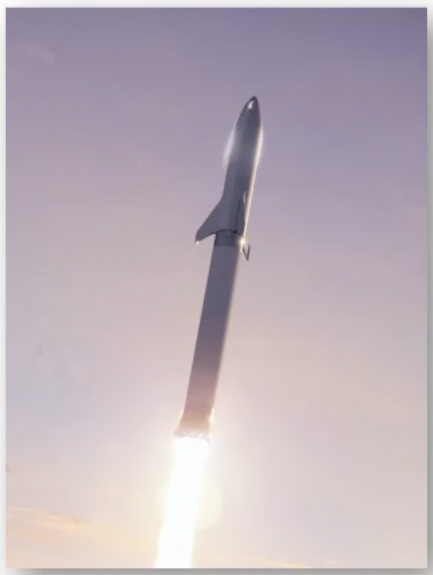
\includegraphics[width=0.25\textwidth]{problema_1.png}
\end{center}
\end{wrapfigure}

El cohete Starship  de la empresa SpaceX  pesa un total de 5000 toneladas métricas cuando está unido a su primera etapa "Super Heavy", y está diseñado con motores capaces de impulsar el conjunto con 74 MN de fuerza. \\¿Qué aceleración puede alcanzar el conjunto? ¿Es dicha aceleración mayor que la gravedad terrestre?\\

\textbf{Formulas base:}\\

Se tomarán las siguientes formulas base de la Dinámica Clásica (Leyes de Newton):

\begin{align}
\boxed{ \vec{F} = m \cdot \vec{a} }\\
\boxed{ 1\,N = 1\,Kg \cdot m/s^2}\\
\boxed{ \vec{P} = m \cdot \vec{g} }\\
\boxed{ \vec{F} = \frac{d\vec{p}}{dt} }
\end{align}

\textbf{Solución:}\\

De la primera ecuación se puede despejar la aceleración, a saber:

\begin{align}
\vec{a} = \frac{\vec{F}}{m} = \frac{74 \times 10^6}{5 \times 10^6} = 14.8\,m/s^2
\end{align}

La aceleración del cohete Starship es $14.8\,m/s^2$, la cual es mayor que la de la gravedad terrestre, lo que le permite elevarse.

%%%%%%%%%%%%%%%%%%%%

\end{document}

